\begin{frame}{Exemplo de handshake assíncrono}
  \begin{center}
  \resizebox{0.85\linewidth}{!}{%
  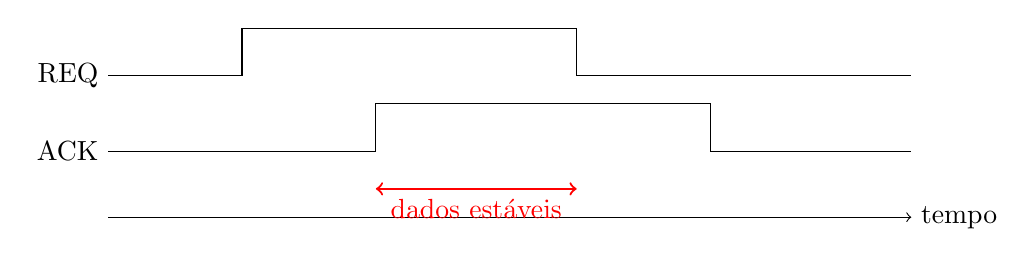
\begin{tikzpicture}[x=0.85cm,y=0.6cm]
    \draw[->] (0,0) -- (12,0) node[right]{tempo};
    \draw (0,3) node[left]{REQ} -- (2,3)--(2,4)--(7,4)--(7,3)--(12,3);
    \draw (0,1.4) node[left]{ACK} -- (4,1.4)--(4,2.4)--(9,2.4)--(9,1.4)--(12,1.4);
    \draw[<->, red, thick] (4,0.6)--(7,0.6) node[midway,below]{dados estáveis};
  \end{tikzpicture}%
  }
  \end{center}
  Sequência típica:
  \begin{enumerate}
    \item a origem coloca o dado e ativa \texttt{REQ};
    \item o destino lê o dado e ativa \texttt{ACK};
    \item a origem desativa \texttt{REQ};
    \item o destino desativa \texttt{ACK}.
  \end{enumerate}
\end{frame}
